	\documentclass[11pt]{article}
	
	\title{Homework 1 - DM CS6220}
	\author{Nakul Camasamudram}
	\usepackage{amsmath,amsfonts,amsthm} % Math packages
	\usepackage{mathtools}
	\usepackage{adjustbox}
	\usepackage{soul}
	%----------------------------------------------------------------------------------------
	%	TITLE SECTION
	%----------------------------------------------------------------------------------------
	
	\newcommand{\horrule}[1]{\rule{\linewidth}{#1}} 
	
	\title{	
	\normalfont \normalsize 
	\textsc{Northeastern University, Data Mining Techniques - CS6220 Fall 2017} \\
	 % Your university, school and/or department name(s)
	\horrule{0.5pt} \\[0.4cm] % Thin top horizontal rule
	\huge Solutions to Homework 2, Part 2 \\ % The assignment title
	\horrule{2pt} \\[0.5cm] % Thick bottom horizontal rule
	}
	\author{Nakul Camasamudram} % Your name
	\date{\normalsize\today} % Today's date or a custom date
	\begin{document}
	
	\maketitle % Print the title
	\newpage
	
	%----------------------------------------------------------------------------------------
	%	PROBLEM 1
	%----------------------------------------------------------------------------------------
	
	\section*{1. K-Means}

	\textbf{Solution:}\\
    
    \begin{itemize}
    	\item \textbf{Iteration 1:} \\
    	The initial centroids are $C_1$ = (2, 10) $C_2$ = (1, 2) $C_3$ = (5, 8). Let D($C_i$) represent the \textbf{euclidean} distance between the respective point and the $i^{th}$ centroid.
    	
		\underline{The $E$-step:} \\
    		\begin{center}
    			\begin{adjustbox}{max width=\textwidth}
				\begin{tabular}{ | c | c | c | c | c |}
	  	 		\hline
    				\textbf{Data Point} & \textbf{D($C_1$)} & \textbf{D($C_2$)} & \textbf{D($C_3$)} & \textbf{Optimal centroid} \\ 
    			\hline
    				(4,9) & 2.23606797749979 & 7.615773105863909 & \textbf{1.4142135623730951} & $C_3$ \\ 
    			\hline
    				(2,10) & \textbf{0.0} & 8.06225774829855 & 3.605551275463989 & $C_1$ \\ 
    			\hline
					(1,2) & 8.06225774829855 & \textbf{0.0} & 7.211102550927978 & $C_2$ \\ 
    			\hline   
    				(2,5) & 5.0 & \textbf{3.1622776601683795} & 4.242640687119285 & $C_2$ \\ 
    			\hline
	    			(6,4) & 7.211102550927978 & 5.385164807134504 & \textbf{4.123105625617661} & $C_3$ \\ 
    			\hline
    				(8,4) & 8.48528137423857 & 7.280109889280518 & \textbf{5.0} & $C_3$ \\ 
    			\hline
    				(7, 5) & 7.0710678118654755 & 6.708203932499369 & \textbf{3.605551275463989} & $C_3$ \\ 
    			\hline 	
    				(5, 8) & 3.605551275463989 & 7.211102550927978 & \textbf{0.0} & $C_3$ \\ 
    			\hline 					
    			\end{tabular}
    			\end{adjustbox}
			\end{center}
		
		\underline{The $M$-step:} \\
		$C_1$ = mean[(2, 10)] = (2.0, 10.0) \\
		$C_2$ = mean[(1, 2), (2, 5)] = (1.5, 3.5) \\
		$C_3$ = mean[(4, 9), (6, 4), (8, 4), (7, 5), (5, 8)] = (6.0, 6.0) \\
		
		\begin{center}
			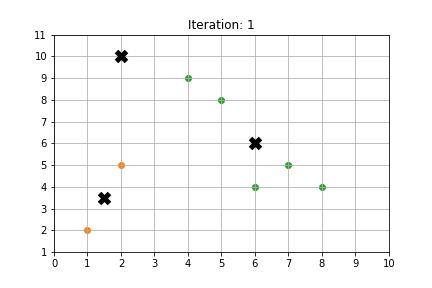
\includegraphics[scale=0.7]{kmeans_graphs/iteration_1.png}
		\end{center}

    	\item \textbf{Iteration 2:} \\
		\begin{center}
			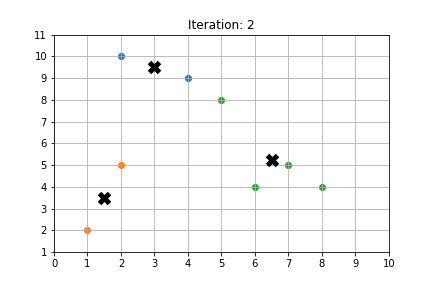
\includegraphics[scale=0.7]{kmeans_graphs/iteration_2.png}
		\end{center}
		
		\item \textbf{Iteration 3:} \\
		\begin{center}
			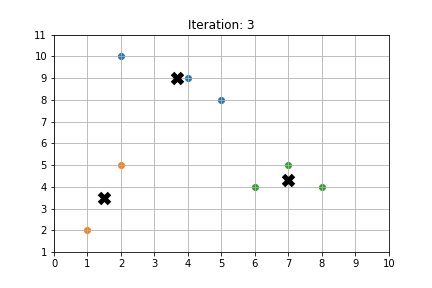
\includegraphics[scale=0.7]{kmeans_graphs/iteration_3.png}
		\end{center}
		
		\item \textbf{Iteration 4:} \\
		\begin{center}
			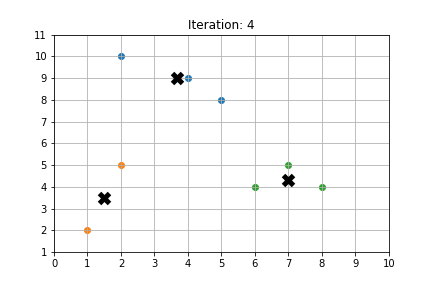
\includegraphics[scale=0.7]{kmeans_graphs/iteration_4.png}
		\end{center}
    \end{itemize}
	\newpage
	
	%----------------------------------------------------------------------------------------
	%	PROBLEM 2
	%----------------------------------------------------------------------------------------
	\section*{2. Agglomerative Hierarchical}

	\textbf{Solution:}\\
	
	\textbf{1. Using MIN as an inter-cluster measure} \\
	
	\textbf{Iteration 1:}
	
	\begin{center}
    	\begin{adjustbox}{max width=\textwidth}
		\begin{tabular}{ | c | c | c | c | c | c | c |}
	  	 	\hline

	  	 	& \textbf{$p_1$} & \textbf{$p_2$} & \textbf{$p_3$} & \textbf{$p_4$} & \textbf{$p_5$} & \textbf{$p_6$}\\
	  	 	\hline
	  	 	
	  	 	\textbf{$p_1$} &  &  &  &  &  &\\
	  	 	\hline
	  	 	
	  	 	\textbf{$p_2$} & 0.2421 &  &  &  &  &  \\
	  	 	\hline
	  	 	
	  	 	\textbf{$p_3$} & 0.2159 & 0.1523 &  &  &  & \\
	  	 	\hline
	  	 	
	  	 	\textbf{$p_4$} & 0.3677 & 0.1965 & 0.1581 &  &  & \\
	  	 	\hline
	  	 	
	  	 	\textbf{$p_5$} & 0.3418 & 0.1334 & 0.2846 & 0.2842 &  & \\
	  	 	\hline	
	  	 	
	  	 	\textbf{$p_6$} & 0.2354 & 0.2530 & \textbf{0.1020} & 0.2195 & 0.3860 & \\
	  	 	\hline			
    		\end{tabular}
    	\end{adjustbox}
	\end{center}
	
	\underline{Cluster 1:} \{3, 6\}
	
	\begin{itemize}
		\item d(\{1\},\{3,6\}) = min(d(\{1\},\{3\}), d(\{1\},\{6\})) = d(\{1\},\{3\})
		\item d(\{2\},\{3,6\}) = min(d(\{2\},\{3\}), d(\{2\},\{6\})) = d(\{2\},\{3\})
		\item d(\{4\},\{3,6\}) = min(d(\{4\},\{3\}), d(\{4\},\{6\})) = d(\{4\},\{3\})
		\item d(\{5\},\{3,6\}) = min(d(\{5\},\{3\}), d(\{5\},\{6\})) = d(\{5\},\{3\})
	\end{itemize}
	
	
	\textbf{Iteration 2:}
	
	\begin{center}
    	\begin{adjustbox}{max width=\textwidth}
		\begin{tabular}{ | c | c | c | c | c | c | c |}
	  	 	\hline

	  	 	& \textbf{$p_1$} & \textbf{$p_2$} & \textbf{$p_3$} & \textbf{$p_4$} & \textbf{$p_5$} & \textbf{$p_6$}\\
	  	 	\hline
	  	 	
	  	 	\textbf{$p_1$} &  &  &  &  &  &\\
	  	 	\hline
	  	 	
	  	 	\textbf{$p_2$} & 0.2421 &  &  &  &  &  \\
	  	 	\hline
	  	 	
	  	 	\textbf{$p_3$} & 0.2159 & 0.1523 &  &  &  & \\
	  	 	\hline
	  	 	
	  	 	\textbf{$p_4$} & 0.3677 & 0.1965 & 0.1581 &  &  & \\
	  	 	\hline
	  	 	
	  	 	\textbf{$p_5$} & 0.3418 & \textbf{0.1334} & 0.2846 & 0.2842 &  & \\
	  	 	\hline	
	  	 	
	  	 	\textbf{$p_6$} & \st{0.2354} & \st{0.2530} & \st{0.1020} & \st{0.2195} & \st{0.3860} & \\
	  	 	\hline			
    		\end{tabular}
    	\end{adjustbox}
	\end{center}
	
	\underline{Cluster 1:} \{3, 6\} \\
	\underline{Cluster 2:} \{2, 5\}
	
	\begin{itemize}
		\item d(\{1\},\{2,5\}) = min(d(\{1\},\{2\}), d(\{1\},\{5\})) = d(\{1\},\{2\})
		\item d(\{4\},\{2,5\}) = min(d(\{4\},\{2\}), d(\{4\},\{5\})) = d(\{4\},\{2\})
		\item d(\{3,6\},\{2,5\}) = min(d(\{3\},\{2\}), d(\{3\},\{5\}), d(\{6\},\{2\}), d(\{6\},\{5\})) = d(\{3\},\{2\})
	\end{itemize}
	
	\textbf{Iteration 3:}
	
	\begin{center}
    	\begin{adjustbox}{max width=\textwidth}
		\begin{tabular}{ | c | c | c | c | c | c | c |}
	  	 	\hline

	  	 	& \textbf{$p_1$} & \textbf{$p_2$} & \textbf{$p_3$} & \textbf{$p_4$} & \textbf{$p_5$} & \textbf{$p_6$}\\
	  	 	\hline
	  	 	
	  	 	\textbf{$p_1$} &  &  &  &  &  &\\
	  	 	\hline
	  	 	
	  	 	\textbf{$p_2$} & 0.2421 &  &  &  &  &  \\
	  	 	\hline
	  	 	
	  	 	\textbf{$p_3$} & 0.2159 & \textbf{0.1523} &  &  &  & \\
	  	 	\hline
	  	 	
	  	 	\textbf{$p_4$} & 0.3677 & 0.1965 & 0.1581 &  &  & \\
	  	 	\hline
	  	 	
	  	 	\textbf{$p_5$} & \st{0.3418} & \st{0.1334} & \st{0.2846} & \st{0.2842} &  & \\
	  	 	\hline	
	  	 	
	  	 	\textbf{$p_6$} & \st{0.2354} & \st{0.2530} & \st{0.1020} & \st{0.2195} & \st{0.3860} & \\
	  	 	\hline			
    		\end{tabular}
    	\end{adjustbox}
	\end{center}
	
	\underline{Cluster 1:} \{3, 6\} \\
	\underline{Cluster 2:} \{2, 5\} \\
	\underline{Cluster 3:} \{\{2, 5\}, \{3, 6\}\} 
	
	\begin{itemize}
		\item d\{\{2, 5, 3, 6\}, \{1\}\} = min(d\{2, 1\}, d\{5, 1\}, d\{3, 1\}, d\{6, 1\}) = d\{3, 1\}
		\item d\{\{2, 5, 3, 6\}, \{4\}\} = min(d\{2, 4\}, d\{5, 4\}, d\{3, 4\}, d\{6, 4\}) = d\{3, 4\}
	\end{itemize}
	
	\textbf{Iteration 4:}
	
	\begin{center}
    	\begin{adjustbox}{max width=\textwidth}
		\begin{tabular}{ | c | c | c | c | c | c | c |}
	  	 	\hline

	  	 	& \textbf{$p_1$} & \textbf{$p_2$} & \textbf{$p_3$} & \textbf{$p_4$} & \textbf{$p_5$} & \textbf{$p_6$}\\
	  	 	\hline
	  	 	
	  	 	\textbf{$p_1$} &  &  &  &  &  &\\
	  	 	\hline
	  	 	
	  	 	\textbf{$p_2$} & \st{0.2421} &  &  &  &  &  \\
	  	 	\hline
	  	 	
	  	 	\textbf{$p_3$} & 0.2159 & \st{0.1523} &  &  &  & \\
	  	 	\hline
	  	 	
	  	 	\textbf{$p_4$} & 0.3677 & \st{0.1965} & \textbf{0.1581} &  &  & \\
	  	 	\hline
	  	 	
	  	 	\textbf{$p_5$} & \st{0.3418} & \st{0.1334} & \st{0.2846} & \st{0.2842} &  & \\
	  	 	\hline	
	  	 	
	  	 	\textbf{$p_6$} & \st{0.2354} & \st{0.2530} & \st{0.1020} & \st{0.2195} & \st{0.3860} & \\
	  	 	\hline			
    		\end{tabular}
    	\end{adjustbox}
	\end{center}
	
	\underline{Cluster 1:} \{3, 6\} \\
	\underline{Cluster 2:} \{2, 5\} \\
	\underline{Cluster 3:} \{\{2, 5\}, \{3, 6\}\} \\
	\underline{Cluster 4:} \{\{2, 5, 3, 6\}, \{4\}\}
	\newpage
	
	
	% ------
	
	\textbf{2. Using MAX as an inter-cluster measure} \\
	
	\textbf{Iteration 1:}
	
	\begin{center}
    	\begin{adjustbox}{max width=\textwidth}
		\begin{tabular}{ | c | c | c | c | c | c | c |}
	  	 	\hline

	  	 	& \textbf{$p_1$} & \textbf{$p_2$} & \textbf{$p_3$} & \textbf{$p_4$} & \textbf{$p_5$} & \textbf{$p_6$}\\
	  	 	\hline
	  	 	
	  	 	\textbf{$p_1$} &  &  &  &  &  &\\
	  	 	\hline
	  	 	
	  	 	\textbf{$p_2$} & 0.2421 &  &  &  &  &  \\
	  	 	\hline
	  	 	
	  	 	\textbf{$p_3$} & 0.2159 & 0.1523 &  &  &  & \\
	  	 	\hline
	  	 	
	  	 	\textbf{$p_4$} & 0.3677 & 0.1965 & 0.1581 &  &  & \\
	  	 	\hline
	  	 	
	  	 	\textbf{$p_5$} & 0.3418 & 0.1334 & 0.2846 & 0.2842 &  & \\
	  	 	\hline	
	  	 	
	  	 	\textbf{$p_6$} & 0.2354 & 0.2530 & \textbf{0.1020} & 0.2195 & 0.3860 & \\
	  	 	\hline			
    		\end{tabular}
    	\end{adjustbox}
	\end{center}
	
	\underline{Cluster 1:} \{3, 6\}
	
	\begin{itemize}
		\item d(\{1\},\{3,6\}) = max(d(\{1\},\{3\}), d(\{1\},\{6\})) = d(\{1\},\{6\})
		\item d(\{2\},\{3,6\}) = max(d(\{2\},\{3\}), d(\{2\},\{6\})) = d(\{2\},\{6\})
		\item d(\{4\},\{3,6\}) = max(d(\{4\},\{3\}), d(\{4\},\{6\})) = d(\{4\},\{6\})
		\item d(\{5\},\{3,6\}) = max(d(\{5\},\{3\}), d(\{5\},\{6\})) = d(\{5\},\{6\})
	\end{itemize}
	
	\textbf{Iteration 2:}
	
	\begin{center}
    	\begin{adjustbox}{max width=\textwidth}
		\begin{tabular}{ | c | c | c | c | c | c | c |}
	  	 	\hline

	  	 	& \textbf{$p_1$} & \textbf{$p_2$} & \textbf{$p_3$} & \textbf{$p_4$} & \textbf{$p_5$} & \textbf{$p_6$}\\
	  	 	\hline
	  	 	
	  	 	\textbf{$p_1$} &  &  &  &  &  &\\
	  	 	\hline
	  	 	
	  	 	\textbf{$p_2$} & 0.2421 &  &  &  &  &  \\
	  	 	\hline
	  	 	
	  	 	\textbf{$p_3$} & \st{0.2159} & \st{0.1523} &  &  &  & \\
	  	 	\hline
	  	 	
	  	 	\textbf{$p_4$} & 0.3677 & 0.1965 & \st{0.1581} &  &  & \\
	  	 	\hline
	  	 	
	  	 	\textbf{$p_5$} & 0.3418 & \textbf{0.1334} & \st{0.2846} & 0.2842 &  & \\
	  	 	\hline	
	  	 	
	  	 	\textbf{$p_6$} & 0.2354 & 0.2530 & \st{0.1020} & 0.2195 & 0.3860 & \\
	  	 	\hline			
    		\end{tabular}
    	\end{adjustbox}
	\end{center}
	
	\underline{Cluster 1:} \{3, 6\} \\
	\underline{Cluster 2:} \{2, 5\}
	
	\begin{itemize}
		\item d(\{1\},\{2,5\}) = max(d(\{1\},\{2\}), d(\{1\},\{5\})) = d(\{1\},\{5\})
		\item d(\{4\},\{2,5\}) = max(d(\{4\},\{2\}), d(\{4\},\{5\})) = d(\{4\},\{5\})
		\item d(\{3, 6\},\{2,5\}) = max(d(\{3\},\{2\}), d(\{3\},\{5\}), d(\{6\},\{2\}), d(\{6\},\{5\})) = d(\{6\},\{5\})
	\end{itemize}
	
	
	\textbf{Iteration 3:}
	
	\begin{center}
    	\begin{adjustbox}{max width=\textwidth}
		\begin{tabular}{ | c | c | c | c | c | c | c |}
	  	 	\hline

	  	 	& \textbf{$p_1$} & \textbf{$p_2$} & \textbf{$p_3$} & \textbf{$p_4$} & \textbf{$p_5$} & \textbf{$p_6$}\\
	  	 	\hline
	  	 	
	  	 	\textbf{$p_1$} &  &  &  &  &  &\\
	  	 	\hline
	  	 	
	  	 	\textbf{$p_2$} & \st{0.2421} &  &  &  &  &  \\
	  	 	\hline
	  	 	
	  	 	\textbf{$p_3$} & \st{0.2159} & \st{0.1523} &  &  &  & \\
	  	 	\hline
	  	 	
	  	 	\textbf{$p_4$} & 0.3677 & \st{0.1965} & \st{0.1581} &  &  & \\
	  	 	\hline
	  	 	
	  	 	\textbf{$p_5$} & 0.3418 & \st{0.1334} & \st{0.2846} & 0.2842 &  & \\
	  	 	\hline	
	  	 	
	  	 	\textbf{$p_6$} & 0.2354 & \st{0.2530} & \st{0.1020} & \textbf{0.2195} & 0.3860 & \\
	  	 	\hline			
    		\end{tabular}
    	\end{adjustbox}
	\end{center}
	
	\underline{Cluster 1:} \{3, 6\} \\
	\underline{Cluster 2:} \{2, 5\} \\
	\underline{Cluster 3:} \{\{3, 6\}, \{4\}\}
	
	\begin{itemize}
		\item d(\{1\},\{3,4,6\}) = max(d(\{1\},\{3\}), d(\{1\},\{4\}), d(\{1\},\{6\})) = d(\{1\},\{4\})
		\item d(\{2,5\},\{3,4,6\}) = max(d(\{2\},\{3\}), d(\{2\},\{4\}), d(\{2\},\{6\}), d(\{5\},\{3\}), d(\{5\},\{4\}), d(\{5\},\{6\})) = d(\{5\},\{6\})
	\end{itemize}
	
	
	\textbf{Iteration 4:}
	
	\begin{center}
    	\begin{adjustbox}{max width=\textwidth}
		\begin{tabular}{ | c | c | c | c | c | c | c |}
	  	 	\hline

	  	 	& \textbf{$p_1$} & \textbf{$p_2$} & \textbf{$p_3$} & \textbf{$p_4$} & \textbf{$p_5$} & \textbf{$p_6$}\\
	  	 	\hline
	  	 	
	  	 	\textbf{$p_1$} &  &  &  &  &  &\\
	  	 	\hline
	  	 	
	  	 	\textbf{$p_2$} & \st{0.2421} &  &  &  &  &  \\
	  	 	\hline
	  	 	
	  	 	\textbf{$p_3$} & \st{0.2159} & \st{0.1523} &  &  &  & \\
	  	 	\hline
	  	 	
	  	 	\textbf{$p_4$} & 0.3677 & \st{0.1965} & \st{0.1581} &  &  & \\
	  	 	\hline
	  	 	
	  	 	\textbf{$p_5$} & \textbf{0.3418} & \st{0.1334} & \st{0.2846} & \st{0.2842} &  & \\
	  	 	\hline	
	  	 	
	  	 	\textbf{$p_6$} & \st{0.2354} & \st{0.2530} & \st{0.1020} & \st{0.2195} & 0.3860 & \\
	  	 	\hline			
    		\end{tabular}
    	\end{adjustbox}
	\end{center}
	
	\underline{Cluster 1:} \{3, 6\} \\
	\underline{Cluster 2:} \{2, 5\} \\
	\underline{Cluster 3:} \{\{3, 6\}, \{4\}\} \\
	\underline{Cluster 4:} \{\{2, 5\}, \{1\}\}
	
	\begin{itemize}
		\item d(\{1\},\{3,4,6\}) = max(d(\{1\},\{3\}), d(\{1\},\{4\}), d(\{1\},\{6\})) = d(\{1\},\{4\})
		\item d(\{2,5\},\{3,4,6\}) = max(d(\{2\},\{3\}), d(\{2\},\{4\}), d(\{2\},\{6\}), d(\{5\},\{3\}), d(\{5\},\{4\}), d(\{5\},\{6\})) = d(\{5\},\{6\})
	\end{itemize}

	
	% --------
	
	\textbf{1. Using AVG as an inter-cluster measure} \\
	
	\textbf{Iteration 1:}
	
	\begin{center}
    	\begin{adjustbox}{max width=\textwidth}
		\begin{tabular}{ | c | c | c | c | c | c | c |}
	  	 	\hline

	  	 	& \textbf{$p_1$} & \textbf{$p_2$} & \textbf{$p_3$} & \textbf{$p_4$} & \textbf{$p_5$} & \textbf{$p_6$}\\
	  	 	\hline
	  	 	
	  	 	\textbf{$p_1$} &  &  &  &  &  &\\
	  	 	\hline
	  	 	
	  	 	\textbf{$p_2$} & 0.2421 &  &  &  &  &  \\
	  	 	\hline
	  	 	
	  	 	\textbf{$p_3$} & 0.2159 & 0.1523 &  &  &  & \\
	  	 	\hline
	  	 	
	  	 	\textbf{$p_4$} & 0.3677 & 0.1965 & 0.1581 &  &  & \\
	  	 	\hline
	  	 	
	  	 	\textbf{$p_5$} & 0.3418 & 0.1334 & 0.2846 & 0.2842 &  & \\
	  	 	\hline	
	  	 	
	  	 	\textbf{$p_6$} & 0.2354 & 0.2530 & \textbf{0.1020} & 0.2195 & 0.3860 & \\
	  	 	\hline			
    		\end{tabular}
    	\end{adjustbox}
	\end{center}
	
	\underline{Cluster 1:} \{3, 6\} \\
	
	\begin{itemize}
		\item d(\{1\},\{3,6\}) = (d(\{1\},\{3\}) + d(\{1\},\{6\})) / (1 x 2) = 0.2256
		\item d(\{4\},\{3,6\}) = (d(\{4\},\{3\}) + d(\{4\},\{6\})) / (1 x 2) = 0.1888
		\item d(\{2\},\{3,6\}) = (d(\{2\},\{3\}) + d(\{2\},\{6\})) / (1 x 2) = 0.2026
		\item d(\{5\},\{3,6\}) = (d(\{5\},\{3\}) + d(\{5\},\{6\})) / (1 x 2) = 0.3353
	\end{itemize}
	
	
	\textbf{Iteration 2:}
	
	\begin{center}
    	\begin{adjustbox}{max width=\textwidth}
		\begin{tabular}{ | c | c | c | c | c | c | c |}
	  	 	\hline

	  	 	& \textbf{$p_1$} & \textbf{$p_2$} & \textbf{$p_3$} & \textbf{$p_4$} & \textbf{$p_5$} & \textbf{$p_6$}\\
	  	 	\hline
	  	 	
	  	 	\textbf{$p_1$} &  &  &  &  &  &\\
	  	 	\hline
	  	 	
	  	 	\textbf{$p_2$} & 0.2421 &  &  &  &  &  \\
	  	 	\hline
	  	 	
	  	 	\textbf{$p_3$} & \st{0.2159} & \st{0.1523} &  &  &  & \\
	  	 	\hline
	  	 	
	  	 	\textbf{$p_4$} & 0.3677 & 0.1965 & \st{0.1581} &  &  & \\
	  	 	\hline
	  	 	
	  	 	\textbf{$p_5$} & 0.3418 & \textbf{0.1334} & \st{0.2846} & 0.2842 &  & \\
	  	 	\hline	
	  	 	
	  	 	\textbf{$p_6$} & \st{0.2354} & \st{0.2530} & \st{0.1020} & \st{0.2195} & \st{0.3860} & \\
	  	 	\hline			
    		\end{tabular}
    	\end{adjustbox}
	\end{center}
	
	\underline{Cluster 1:} \{3, 6\} \\
	\underline{Cluster 2:} \{2, 5\} \\
	
	
	\begin{itemize}
		\item d(\{1\},\{2,5\}) = avg(d(\{1\},\{2\}), d(\{1\},\{5\})) = 0.2919
		\item d(\{4\},\{2,5\}) = avg(d(\{2\},\{4\}), d(\{2\},\{5\})) = 0.1649
		\item d(\{3,6\},\{2,5\}) = avg(d(\{3\},\{2\}), d(\{3\},\{5\}), d(\{6\},\{2\}), d(\{6\},\{5\})) = 0.2689
	\end{itemize}
	
	
	\textbf{Iteration 3:}
	
	\begin{center}
    	\begin{adjustbox}{max width=\textwidth}
		\begin{tabular}{ | c | c | c | c | c | c | c |}
	  	 	\hline

	  	 	& \textbf{$p_1$} & \textbf{$p_2$} & \textbf{$p_3$} & \textbf{$p_4$} & \textbf{$p_5$} & \textbf{$p_6$}\\
	  	 	\hline
	  	 	
	  	 	\textbf{$p_1$} &  &  &  &  &  &\\
	  	 	\hline
	  	 	
	  	 	\textbf{$p_2$} & \st{0.2421} &  &  &  &  &  \\
	  	 	\hline
	  	 	
	  	 	\textbf{$p_3$} & \st{0.2159} & \st{0.1523} &  &  &  & \\
	  	 	\hline
	  	 	
	  	 	\textbf{$p_4$} & 0.3677 & \st{0.1965} & \st{0.1581} &  &  & \\
	  	 	\hline
	  	 	
	  	 	\textbf{$p_5$} & \st{0.3418} & \st{0.1334} & \st{0.2846} & \textbf{0.2842} &  & \\
	  	 	\hline	
	  	 	
	  	 	\textbf{$p_6$} & \st{0.2354} & \st{0.2530} & \st{0.1020} & \st{0.2195} & \st{0.3860} & \\
	  	 	\hline			
    		\end{tabular}
    	\end{adjustbox}
	\end{center}
	
	\underline{Cluster 1:} \{3, 6\} \\
	\underline{Cluster 2:} \{2, 5\} \\
	
	
	\begin{itemize}
		\item d(\{1\},\{2,5\}) = avg(d(\{1\},\{2\}), d(\{1\},\{5\})) = 0.2919
		\item d(\{4\},\{2,5\}) = avg(d(\{2\},\{4\}), d(\{2\},\{5\})) = 0.1649
		\item d(\{3,6\},\{2,5\}) = avg(d(\{3\},\{2\}), d(\{3\},\{5\}), d(\{6\},\{2\}), d(\{6\},\{5\})) = 0.2689
	\end{itemize}
%----------------------------------------------------------------------------------------
	%	PROBLEM 3
	%----------------------------------------------------------------------------------------
	\section*{3. DBSCAN}

	\textbf{Solution:}\\
	\newpage
\end{document}




























